\documentclass[11pt, a4paper]{article}

\usepackage{graphicx}
\usepackage[a4paper,top=3cm,bottom=2cm,left=2cm,right=2cm,marginparwidth=1.75cm]{geometry}
\usepackage[english]{babel}
\usepackage[utf8x]{inputenc}
\usepackage{subfig}
\usepackage{float}
\usepackage{amsmath}
\usepackage{amssymb}
\usepackage{mhchem}
\usepackage{hyperref}
\usepackage{tikz}
\usepackage{cancel}

\graphicspath{ {./images} }
\newcommand*{\qed}{\hfill\ensuremath{\quad\square}}%
\newcommand*{\rad}{\ensuremath{\,\text{rad}}}
\newcommand*{\R}{\ensuremath{\mathbb{R}}}
\newcommand*{\C}{\ensuremath{\mathbb{C}}}
\renewcommand*{\Re}{\operatorname{Re}}
\renewcommand*{\Im}{\operatorname{Im}}
\renewcommand*{\epsilon}{\varepsilon}
\renewcommand*{\phi}{\varphi}

\makeatletter
\renewcommand*\env@matrix[1][*\c@MaxMatrixCols c]{%
  \hskip -\arraycolsep
  \let\@ifnextchar\new@ifnextchar
  \array{#1}}
\makeatother

\newtheorem{theorem}{Theorem}

%------------------------------------------------
%Templates for images and figures
% \begin{figure}[h]
%   \centering
%   \subfloat[caption 1]{{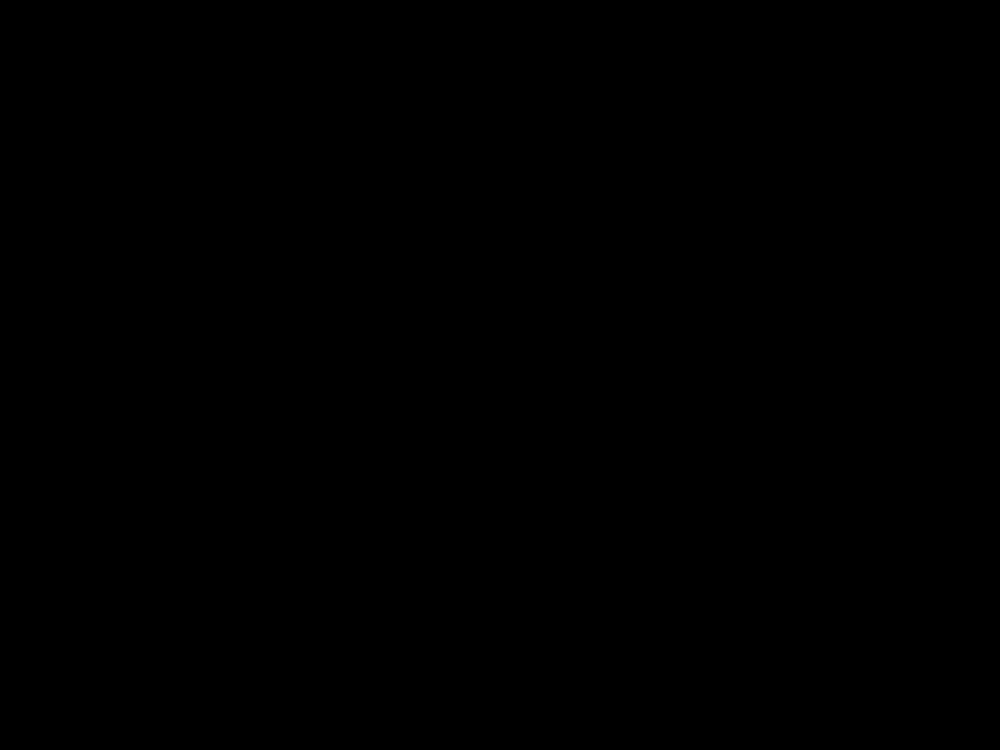
\includegraphics[width=30mm]{images/placeholder.png}}}%
%   \qquad
%   \subfloat[caption 2]{{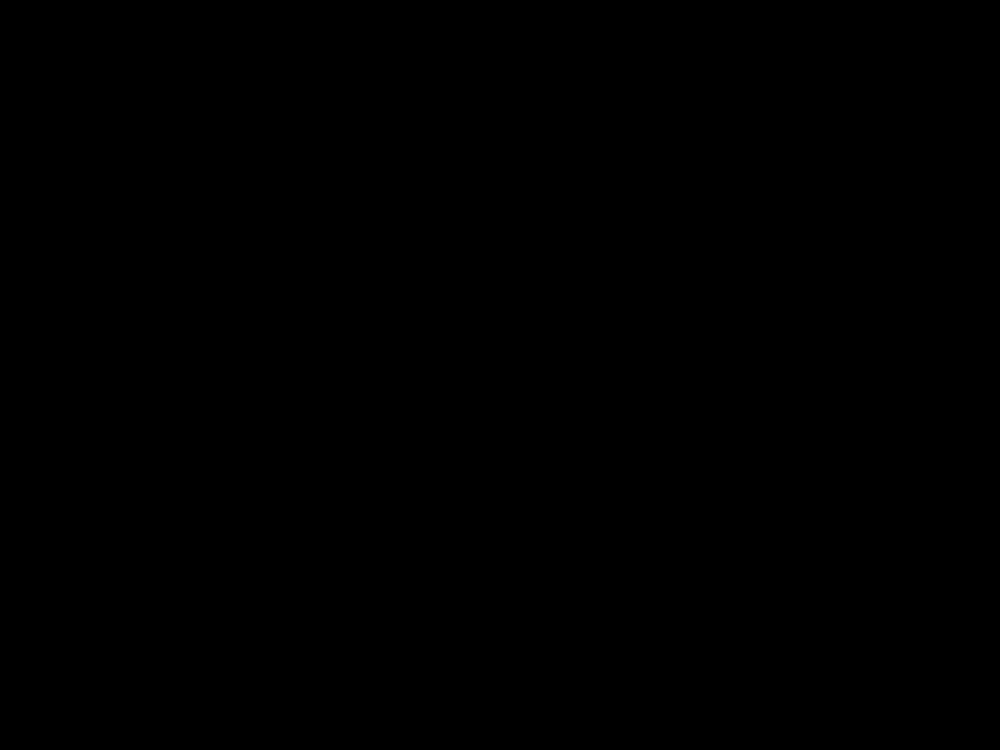
\includegraphics[width=30mm]{images/placeholder.png}}}%
%   \caption{Description}
% \end{figure}

% \begin{figure}[h]
%   \centerline{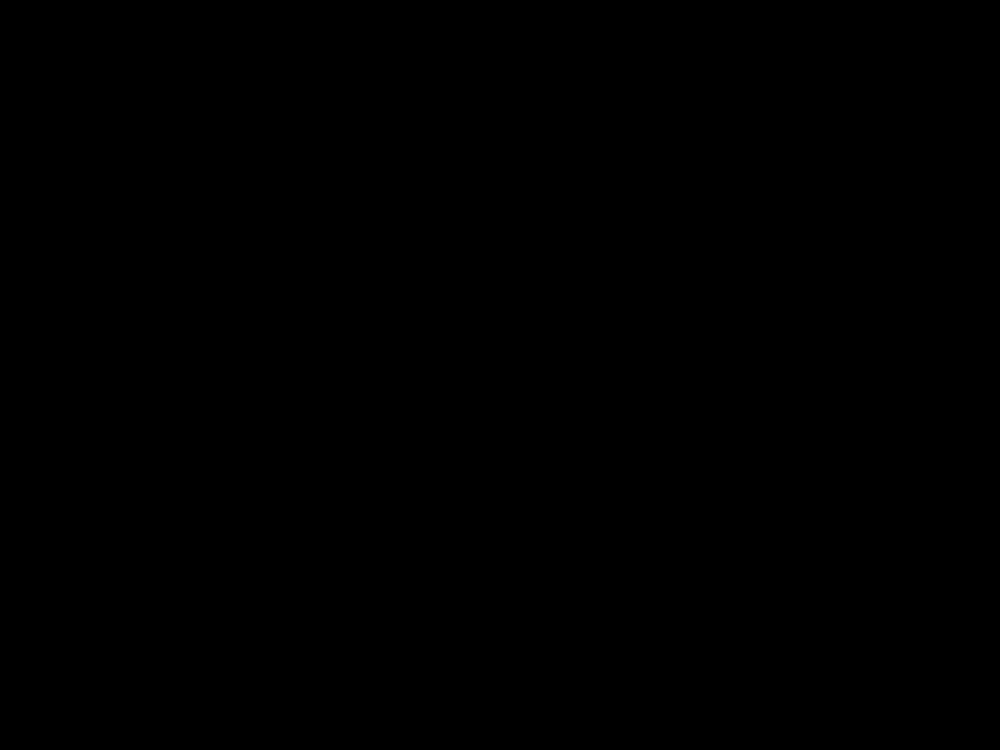
\includegraphics[width=50mm]{images/placeholder.png}}
%   \caption{Description}
% \end{figure}

%Template for a simple table 
%\begin{table}[h]
%   \caption{Description} %title of the table
%   \centering % centering table
%   \begin{tabular}{l rr} % creating three columns
%     \hline\hline %inserting double-line
%     & & \\ [0.5ex] % Insert half line vertical spacing
%     \hline % inserts single-line
%     & & \\ 
%     & & \\
%     & & \\
%     & & \\
%   \hline % inserts single-line
%   \end{tabular}
%   \label{tab:hresult}
% \end{table}
%-----------------------------------------------

\begin{document}
\setcounter{section}{5} 
\setcounter{equation}{0}

\section{WOP3B Lecture 6: Fatigue of rotary equipment (14/05/2020)}


\subsection{Safe life Design vs. Infinite Life Design}
The previous lecture on fatigue covered safe life design for products and parts using rain-flow counting and the Palmgren-Miner rule. This lecture will cover infinite life design of primarily rotary equipment. SLd means designing parts that will not fail to fatigue in the life span of the product. Infinite life design means designing parts that will never fail to fatigue. This can be achieved by considering the endurance limit\footnote{The endurance limit was briefly discussed in the fatigue level 1 lecture} for the material. The process revolves around designing parts such that $\sigma_{von\;mises} \leq \sigma_e$, where $\sigma_e$ is the endurance limit of the part. ILD is important to consider for rotary equipment such as axles since $10^7$ is not that much when rotating at $2000+\,rpm$. For reference at $2000\,rpm$ the $10^7$ cycles mark would be reached in roughly $84$ hours. This excludes SLD as an option since all machines would probably need to oeprate more then a couple of days before running the risk of failure.


\subsection{The rotary bending test}
The endurance limit of an a shaft is usually found empirically. The standardized test for this is the rotary bending test. The test is basicly applying a known bending load to an axle and spinning it around a bunch untill it breaks. Doing a rotary bending test is usually very expensive and time consuming as $10^7$ cycles are reached in about $60$ hours at $2500-3000\,rpm$. Doing the test is not enough to gain an answer with any sort of confidence and running the test 10 times takes alot of time even when several are run in parallel. This also means the value for the endurance limit found by a rotary bending test is usually a linear regression of all tests done.
\begin{figure}[h]
  \centerline{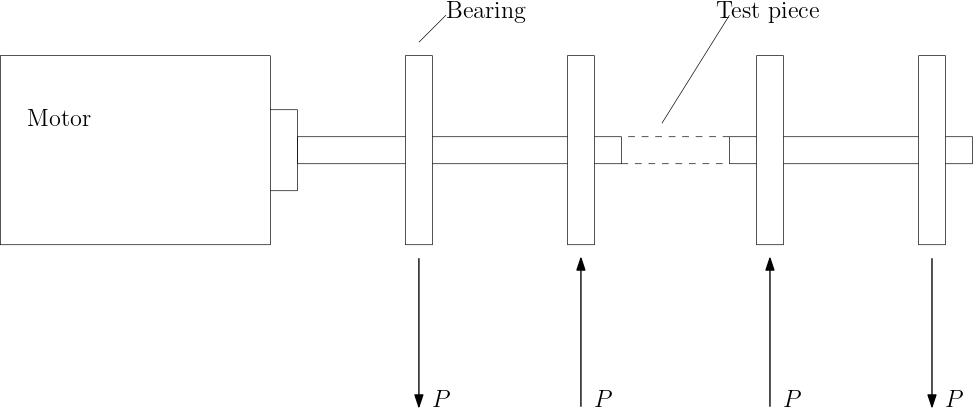
\includegraphics[width=80mm]{images/RotaryTest.png}}
  \caption{A typical rotary bending test setup where the load applied $P$ is some known quantity.}
\end{figure}


\subsection{The reliabilty factor}
As noted before the endurance limit data found in tables and databases is usually a mean value. We usually assume standard deviation from the reported value rarely exceeds $8\%$, which is to say: $\sigma = 0.08\mu$ where $\sigma$ is the standard deviation and $\mu$ the expected value. The reliability factor can then be found by the follwing expression:
\begin{equation}
  C_{reliab} = \frac{\mu - z\sigma}{\mu}
\end{equation}
Where $z$ is the standard scores. The standard score $z$ is a variable depending on the standard deviation and the expected value. It can be computed using the probabilty density function but it is easier to look up a given $z$ value for the corresponding failure rate. When Failure rate is $5\%$ the $R(t)$ value will be $95\%$ which corresponds to a $z$-score of $1.64$. Thus the reliability factor will become:
\begin{equation}
  C_{reliab} = \frac{\mu - 1.64\cdot 0.08\mu}{\mu} = 0.87
\end{equation}
The endurance limit corrected for reliability as then given as:
\begin{equation}
  \sigma_e = C_{reliab}\sigma_e'
\end{equation}
The value $\sigma_e'$ is the value for the endurance limit found in tables.


\subsection{Estimating the endurance limit of parts}
There are many factors that go into determining the final endurance limit of a part. The total expression involving all factors is as follows:
\begin{equation}
  \sigma_e = C_{load}C_{size}C_{surf}C_{temp}C_{reliab}\sigma_e'
\end{equation}
\begin{itemize}
\item Load factor ($C_{load}$): a factor depending on the type of load applied to a part.
\end{itemize}
\begin{equation}
  C_{load} = \begin{cases}
    = 1,\quad \text{Bending}\\
    = 0.7,\quad \text{Axial loading}\\
    = 0.58,\quad \text{Pure torsion}
  \end{cases}
\end{equation}
\begin{itemize}
  \item Size factor ($C_{size}$): The test specimens are usually small ($\approx\,8\,mm$). Large parts will fail at lower stresses then the small test parts, thus the size factor is introduced to correct for this. 
\end{itemize}
\begin{equation}
  C_{size} = \begin{cases}
    = 1,\quad d \leq 8\,mm\\
    = 1.189d^{-0.097},\quad 8\,mm \leq d \leq 250\,mm\\
    = 0.6,\quad d > 250\,mm
  \end{cases}
\end{equation}
\begin{itemize}
  \item Surface factor ($C_{surf}$): Surface roughness reduces the fatigue strength. The expression for the value of the surface factor is given by $C_{surf} = 1 - 0.22\log(R_z)\left(\log\left(\frac{R_m}{20}\right) - 1 \right)$ Where $R_z = 7.5R_a$ per DIN norm and $R_a$ the surface roughness in $\mu m$. $R_m$ is the UTS\footnote{Ultimate Tensile Strength} of the material.
  \item Temperature factor ($C_{temp}$): High temperatures increase the toughness of materials. conversly very low temperatures increase the brittleness of materials. For ambient temperatures $C_{temp} = 1$. It can otherwise be found in tables for applicable circumstances.
\end{itemize}
As a general rule of thumb after applying all the correction factors:
\begin{equation}
  \sigma_e \approx \frac{1}{3}R_m
\end{equation}


\subsection{Stress concentration factors as applied to the endurance limit}
As we know sudden changes in geometry lead to an increase in local stress in a material. The amount of stress increased is quantified by $K_t$, the stress concentration factor. It can be either computed or found using FEM analysis as follos:
\begin{equation}
  K_t = \frac{\sigma_{max}}{\sigma_{nominal}}
\end{equation}
The value for $K_t$ can also be found in tables or literature for common geometries. Stress concentrations can be relieved in several ways. The most common ones are introducing a greater radius, making the jump in geometry less sudden, and introducing a stress relief groove.
\begin{figure}[h]
  \centerline{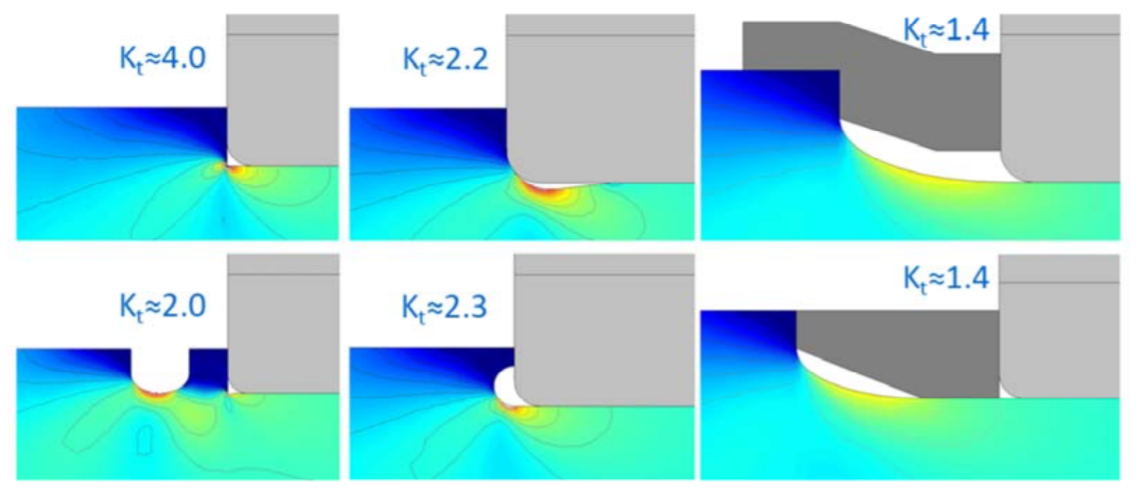
\includegraphics[width=100mm]{images/KtVals.png}}
  \caption{Visualization of typical methods of reducing stress concentrations}
\end{figure}
The value for $K_t$ is purely determined by geometry. This means the value does not take variations in material properties into account. An example of why this is relevant: Softer materials will start plastic deformation earlier then harder materials. Because of this the stress-strain curve is more flattened compared to the harder material. Because of this relation the actual stress concentration would be lower then what the value $K_t$ would predict. The stress intensity factor that \underline{does} take into account these material properties is usually denoted as $K_f$. Since it takes into account more then just geometry we can say that by definition:
\begin{equation}
  K_f \leq K_t
\end{equation}
This means using the value for $K_t$ would always be considered safe as it will lead to a higher result then what we observe in reality.


\subsection{Case study: Weight saving}
Consider 2 axles. One with a $20\,mm$ diameter and one with a $12\,mm$ diameter. The $20\,mm$ axle has a groove of $0.5\,mm$ cut into the axle for a retaining ring. We want to know which axle can be loaded most in rotary bending test.
\begin{figure}[h]
  \centering
  \subfloat[Axle 1]{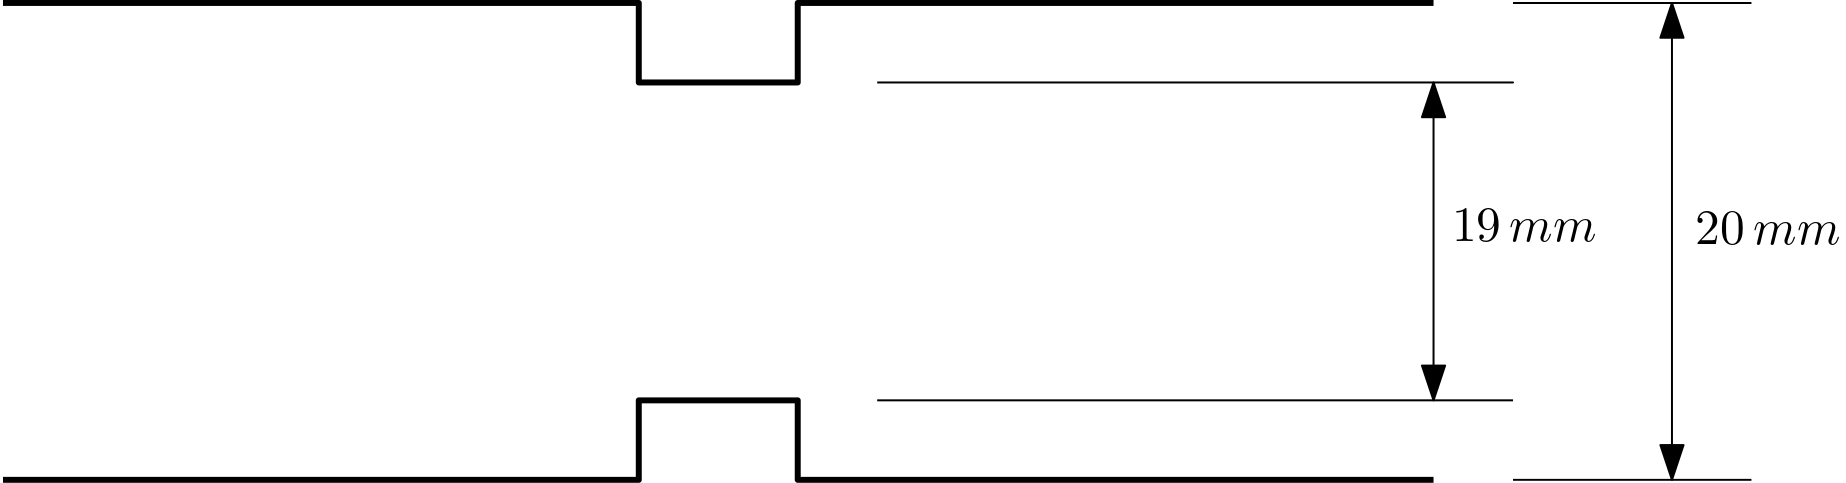
\includegraphics[width=60mm]{images/Axle1.png}}
  \qquad \qquad
  \subfloat[Axle 2]{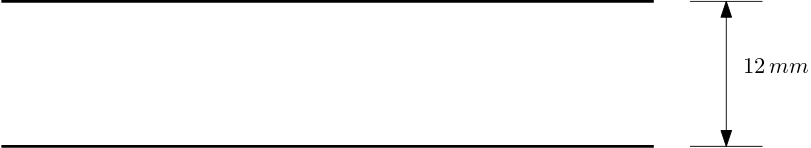
\includegraphics[width=60mm]{images/Axle2.png}}
  \caption{The 2 axles being considered for the case study.}
\end{figure} 
We first consider the strength under static loading:
\begin{gather*}
  M_{12} = \frac{\pi}{32}d_{12}^3\sigma\\
  M_{20} = \frac{\pi}{32}d_{19}^3\sigma
\end{gather*}
The ratio between these 2 acceptable bending loads then becomes:
\begin{equation*}
  \frac{M_{12}}{M_{20}} = \left(\frac{d_{12}}{d_{19}}\right)^3 \approx 0.252
\end{equation*}
Thus the maximum static bending load which can be applied on the smaller axle is about $25\%$ that of the maximum bending load which can be applied to the $20\,mm$ axle. We now consider the dynamic loading on the axles. We assume that for the small groove $K_t \approx 5$. Then:
\begin{gather*}
  M_{12} = \frac{\pi}{32} d_{12}^3 \sigma_e\\
  M_{20} = \frac{\pi}{32} d_{19}^3 \frac{\sigma_e}{K_t}
\end{gather*}
The new ratio between the 2 under dynamic loading then becomes:
\begin{equation*}
  \frac{M_{12}}{M_{20}} = \frac{d_{12}^3}{d_{19}^3 / K_t} \approx 1.26
\end{equation*}
This means the $12\,mm$ axle can widthstand a roughly $26\%$ higher bending load under dynamic loading. Thus interestingly if considering a static load the $12\,mm$ axles in only about $\frac{1}{4}$ the strength of the thicker $20\,mm$ axle. However when we consider a dynamic loading, and take into account the stress concentration raised by the groove we find that the smaller axle can widthstand a much higher bending load.
\end{document}